\section{VL 03: Einfluss von IT-Systemen auf Geschäftsmodelle}

In dieser Vorlesung ging es hauptsächlich um die Veränderung eines Geschäftsmodells durch IT. Zunächst einmal wird der Markt für ein Produkt durch verschiedene Aspekte beeinflusst:

\begin{itemize}

    \item Substitute (d.h. Ersatzprodukte)

    \item Kundeneinfluss

    \item Lieferanteneinfluss

    \item Markteintritte (Neue Produkte / Unternehmen)

\end{itemize}

Um ein Geschäftsmodell besser beschreiben zu können, wurde das "Business Canvas Model" eingeführt:

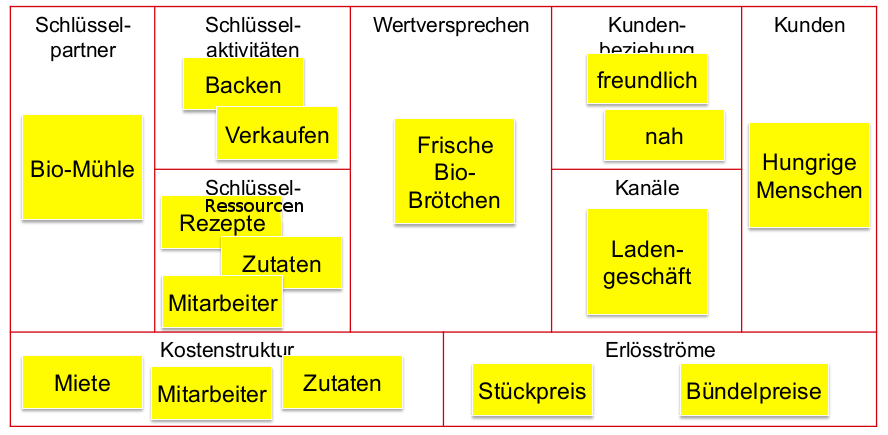
\includegraphics[scale=0.5]{BCM.png}

\newpage

Die IT nimmt auf jeden der Aspekte im Diagramm auf verschiedene Arten und Weisen Einfluss:

\begin{description}

    \item[Schlüsselpartner]

    \item Vereinfachte Einbindung von Partnern

    \item digitale Partner (Suchmaschinen)

    \item[Schlüsselaktivitäten]

    \item Automatisierung

    \item Beschleunigung

    \item Tracking, Überwachung

    \item[Schlüsselressorucen]

    \item Information

    \item Informationssysteme

    \item Informations und Kommunikations Infrastruktur

    \item (offene) It-Schnittstellen

    \item[Wertversprechen]

    \item Besser Informationen und Kommunikation

    \item Informationsbasierte Produkte/Dienstleistungen

    \item Günstigere, schnellere Leistungen

    \item[Kundenbeziehung]

    \item Websites, und Apps.

    \item Selbstbedienung

    \item Nutzergenrierte Inhalte

    \item Communities

    \item[Kanäle]

    \item Electronic- und Mobile-Commerce

    \item Intermediation: Etablierung eines neuen Mittlers.

    \item Reintermediation: Erneute Etablierung eines Mittlers 

    \item[Kunden]

    \item Veränduerung von Zielgruppen etc. (auch international)

    \item[Erlösströme]

    \item Nutzungsabhängige Preise ("Pay-per-use")

    \item Indirekte Erlöse (Daten verkaufen, Crapware installieren, Werbung)

    \item[Kostenstrucktur]

    \item geringere Transaktionskosten

    \item Vereinfachtes Verteilen von Risiken.

\end{description}

Insgesamt werden Geschäftsmodelle durch IT umfangreich verändert, dabei geht es besonders um \textbf{Vermittlung Koordination} von Dienstleistungen und Produkten. Sowie um die erschließung textbf{neuer Partner} (viele kleine Anbieter).